\documentclass{article}
%\usetheme{default}
\usepackage{geometry}

\usepackage{amsmath}
\usepackage{amssymb}
\usepackage{tikz}
\usetikzlibrary{shapes, arrows}

\begin{document}
%	\begin{frame}{Analysis Strategy and -Setup}
	\begin{center}
		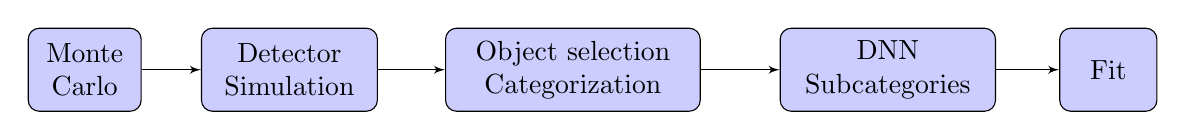
\begin{tikzpicture}
			\tikzstyle{terminator} = [rectangle, draw, text centered, rounded corners, minimum height=3em]
			\tikzstyle{connector} = [draw, -latex']
			\node [terminator, fill=blue!20, text width=1.2cm] at (0,0) (start) {Monte Carlo};
			\node [terminator, fill=blue!20, text width=2cm] at (2.6,0) (detector) {Detector Simulation};
			\node [terminator, fill=blue!20, text width = 3cm] at (6.2,0) (cat) {Object selection\\Categorization};
			\node [terminator, fill=blue!20, text width = 2.5cm] at (10.2,0) (dnn) {DNN\\Subcategories};
			\node [terminator, fill=blue!20, text width = 1cm] at (13,0) (fit) {Fit};
			\path [connector] (start) -- (detector);
			\path [connector] (detector) -- (cat);
			\path [connector] (cat) -- (dnn);
			\path [connector] (dnn) -- (fit);
		\end{tikzpicture}
	\end{center}
%\end{frame}
\end{document}
